\subsection*{Log ind}
I systemet benyttes en log ind funktion til at beskytte og identificere den enkelte bruger. Brugeren vil her angive log ind-information, der vil tillade adgang til information i form af private oplysninger og tidligere resultater, tilknyttet den givne bruger. Aktiviteterne for log ind fremgår af \autoref{fig:logind}.    


\begin{figure} [H]
\centering
\textbf{Aktivitetsdiagram: Log ind}\par\medskip
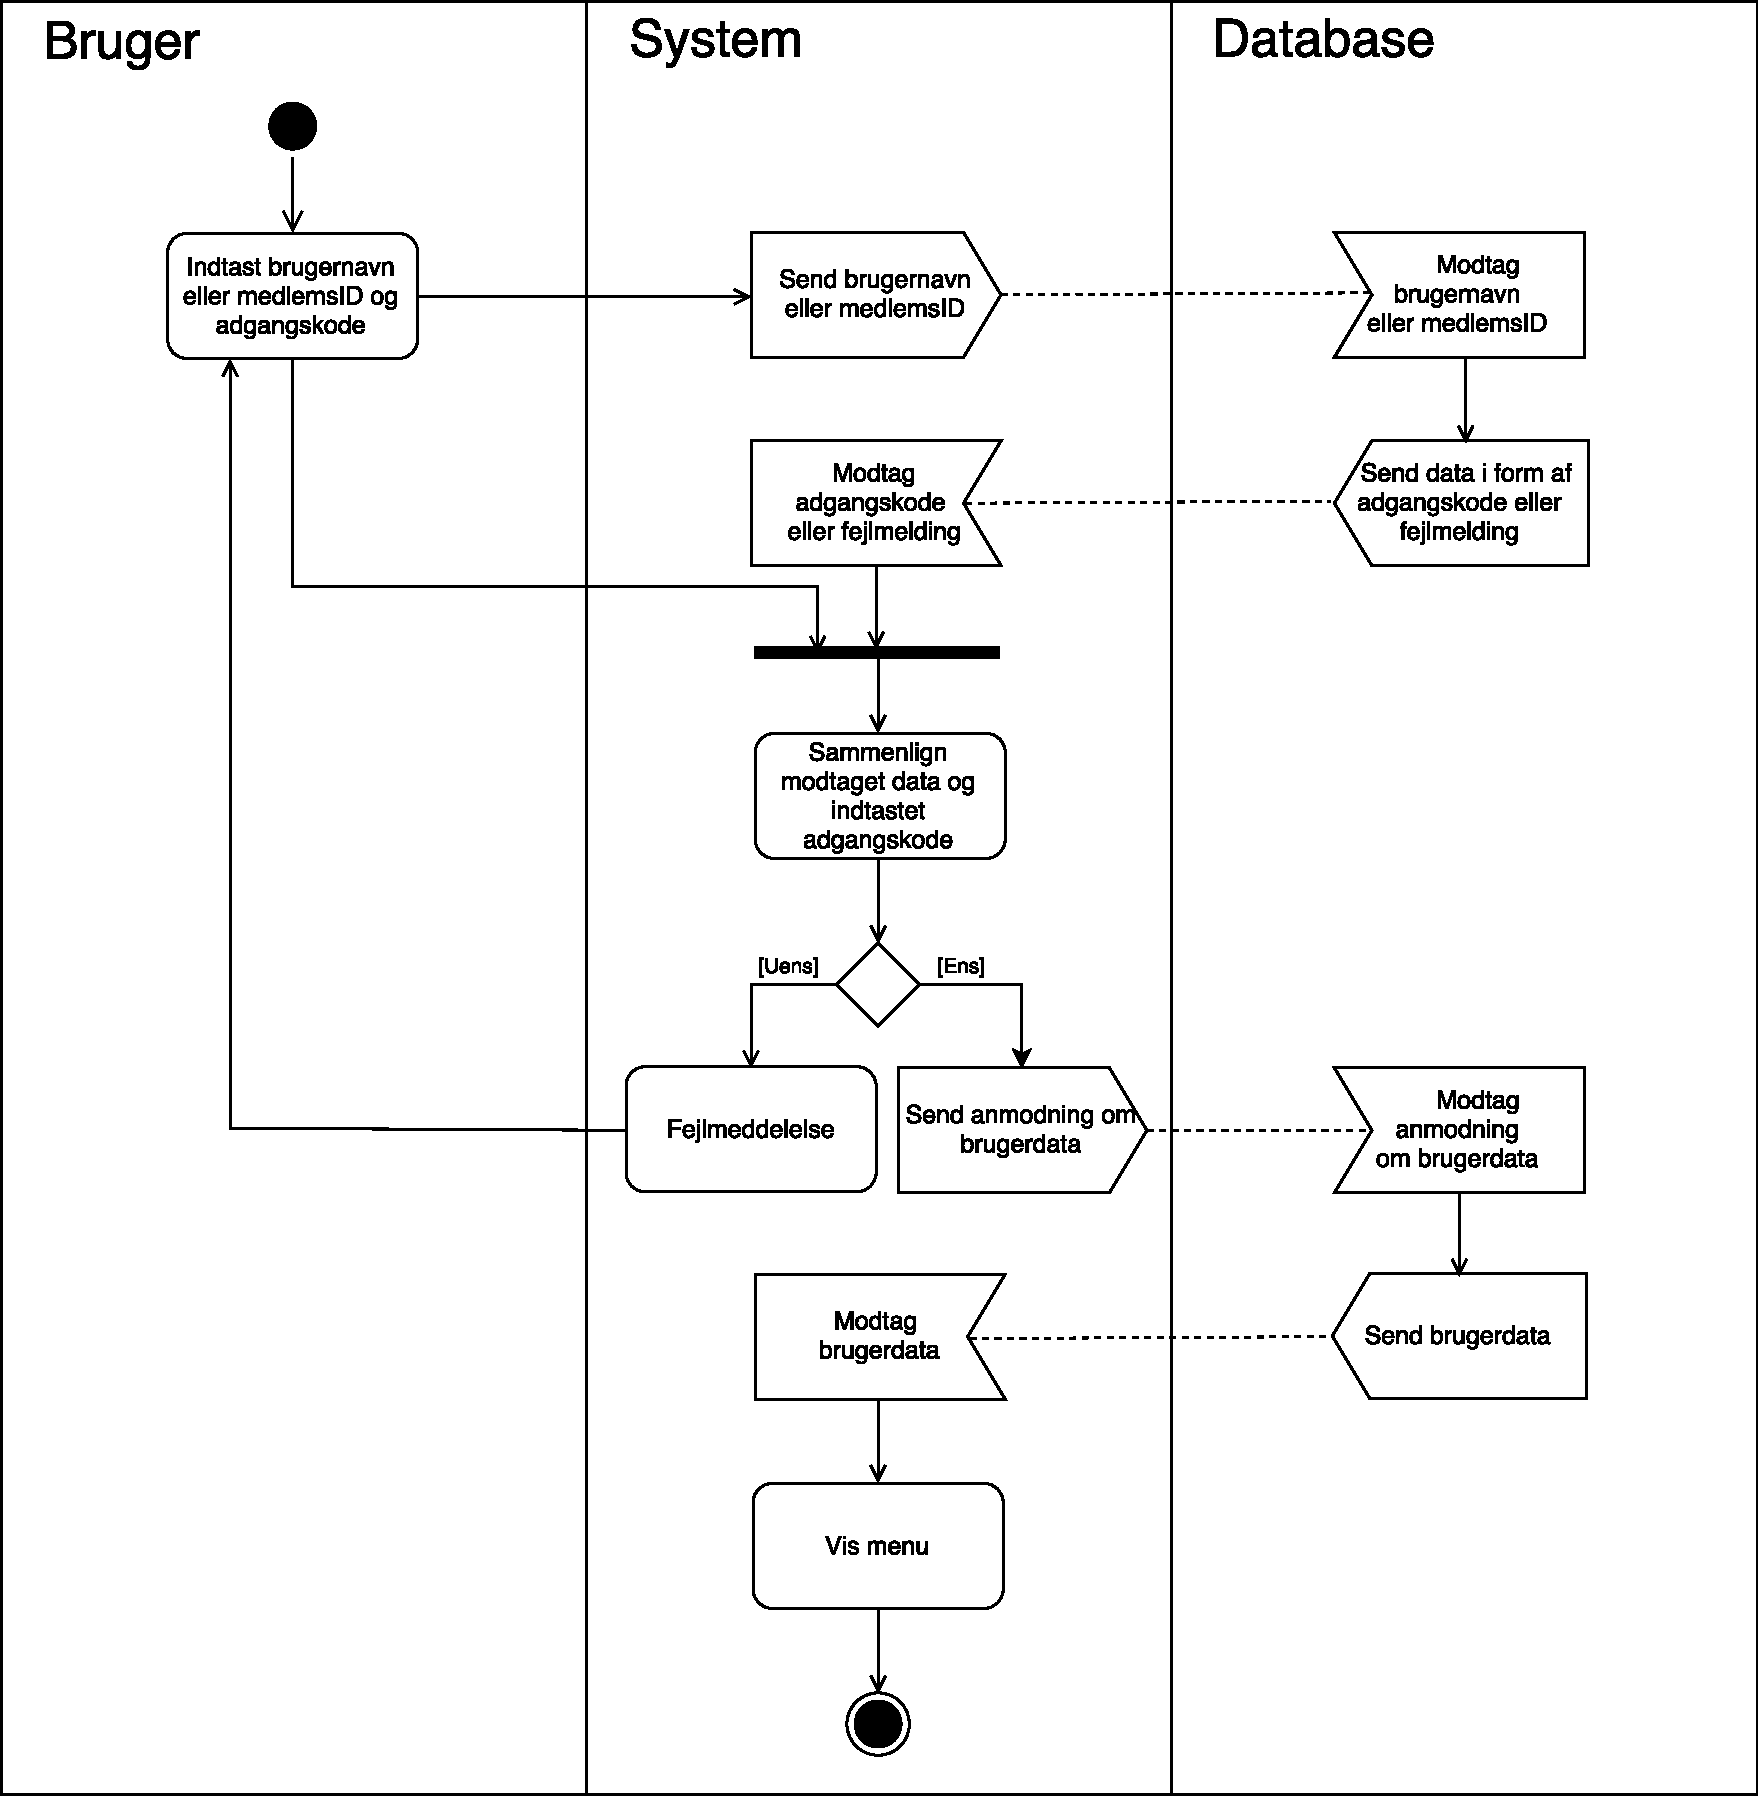
\includegraphics[width=0.7\textwidth]{figures/aktivitetsdiagram/Logind}
\caption{Aktivitetsdiagram for log ind. Kategorisering af KOL uddybes af \autoref{fig:Kate}}
\label{fig:logind}
\end{figure}


\noindent
Når KOL-patienten vil anvende app'en fremgår en grænseflade for log ind, hvor brugeren kan angive medlemsID og adgangskode. Systemet sender det indtastede medlemsID til en database, som tilbagesender det tilhørende adgangskode, hvis det findes i databasen. Findes de indtastede informationer ikke, sendes en fejlmeddelelse og brugeren returneres til grænsefladen for log ind. Hvis brugeren ikke er oprettet i databasen skal den kontakte sundhedspersonalet. 
Findes de indtastede informationer i databasen validerer systemet den angivne adgangskode med den modtaget adgangskode. Er disse ikke ens vises en fejlmeddelelse og brugeren returneres til grænsefladen for log ind. Har brugeren glemt adgangskoden skal de kontakte sundhedspersonalet. Hvis de er ens anmoder systemet om at hente brugerdata i databasen, herunder brugerens informationer og tidligere resultater. Mislykkes dette sendes og vises en fejlmeddelelse. Lykkes dette modtages brugerdata.
Herefter anmoder systemet om kategorisering i databasen. Findes denne ikke sendes en fejlmeddelelse og systemet viser kategorisering, som brugeren skal angive. Kategoriseringen fremgår af \autoref{fig:Kate} Er der tidligere foretaget en kategorisering vises hovedmenuen.

%Idet brugeren åbner app'en, vil en grænseflade for log ind vises. Hertil er det ikke muligt at gå videre gennem aktiviteterne før brugeren har angivet log ind-information i form af medlemsID og en adgangskode. 
%Såfremt at medlemsID'et findes, benyttes det efterfølgende i databasen til at identificere den korrekte adgangskode og returnere denne til systemet. Findes medlemsID'et ikke vil dette resultere i at systemet vil vise en fejlmeddelelse, og returnere til grænsefladen for log ind. 
%Idet den korrekte adgangskode modtages af systemet, sammenlignes denne med angivet adgangskode. I tilfælde af at adgangskoderne ikke er identiske, vises en fejlmeddelelse og systemet returnere til grænsefladen for log ind. Er adgangskoderne identiske vil systemet hente alt brugerrelateret information fra databasen. I tilfælde af at data'en ikke modtages vises en fejlmeddelelse, ellers tjekkes om det er første gang brugeren logger ind på appen. 
%Ved førstegangs log ind vil systemet udføre en aktivitet, hvorigennem systemet får angivet brugerens kategorisering af KOL. Efter angivelsen af kategoriseringen, eller ved efterfølgende log ind vil systemet gå direkte til at vise hovedmenuen.  
   


